\section{Resultados y discusión}
\label{sec:resultados}

Los resultados se presentan en el orden de las fases del proyecto: caracterización del canal (Fase~1), diseño y validación del sistema Tx--canal--Rx (Fase~2), configuración de la interfaz SDR (Fase~3) y medición de curvas BER (Fase~4). Todas las figuras de GNU Radio son capturas de los flujogramas del grupo en ejecución; las capturas completas de cada prueba están en el Anexo~\ref{app:capturas}.

\subsection{Fase 1: caracterización del canal con ruido impulsivo}
En la primera fase se partió del flujograma base del curso y se modificó para el escenario S1 (Anexo~\ref{app:fase1}): la tabla de símbolos pasó de OOK a BPSK $(-1,+1)$ y se agregó un tren de impulsos reales de amplitud $A_{imp}$, uno cada 256 muestras (1~ms), sumado a la salida del AWGN. En esta fase el pulso era rectangular de 8 muestras y no había receptor; se observaron la señal temporal, la constelación de las muestras y la PSD para la referencia y para las tres severidades de la Tabla~\ref{tab:fase1}, con $R_s$, SPS y $f_s$ fijos.

\begin{figure*}[t]
    \centering
    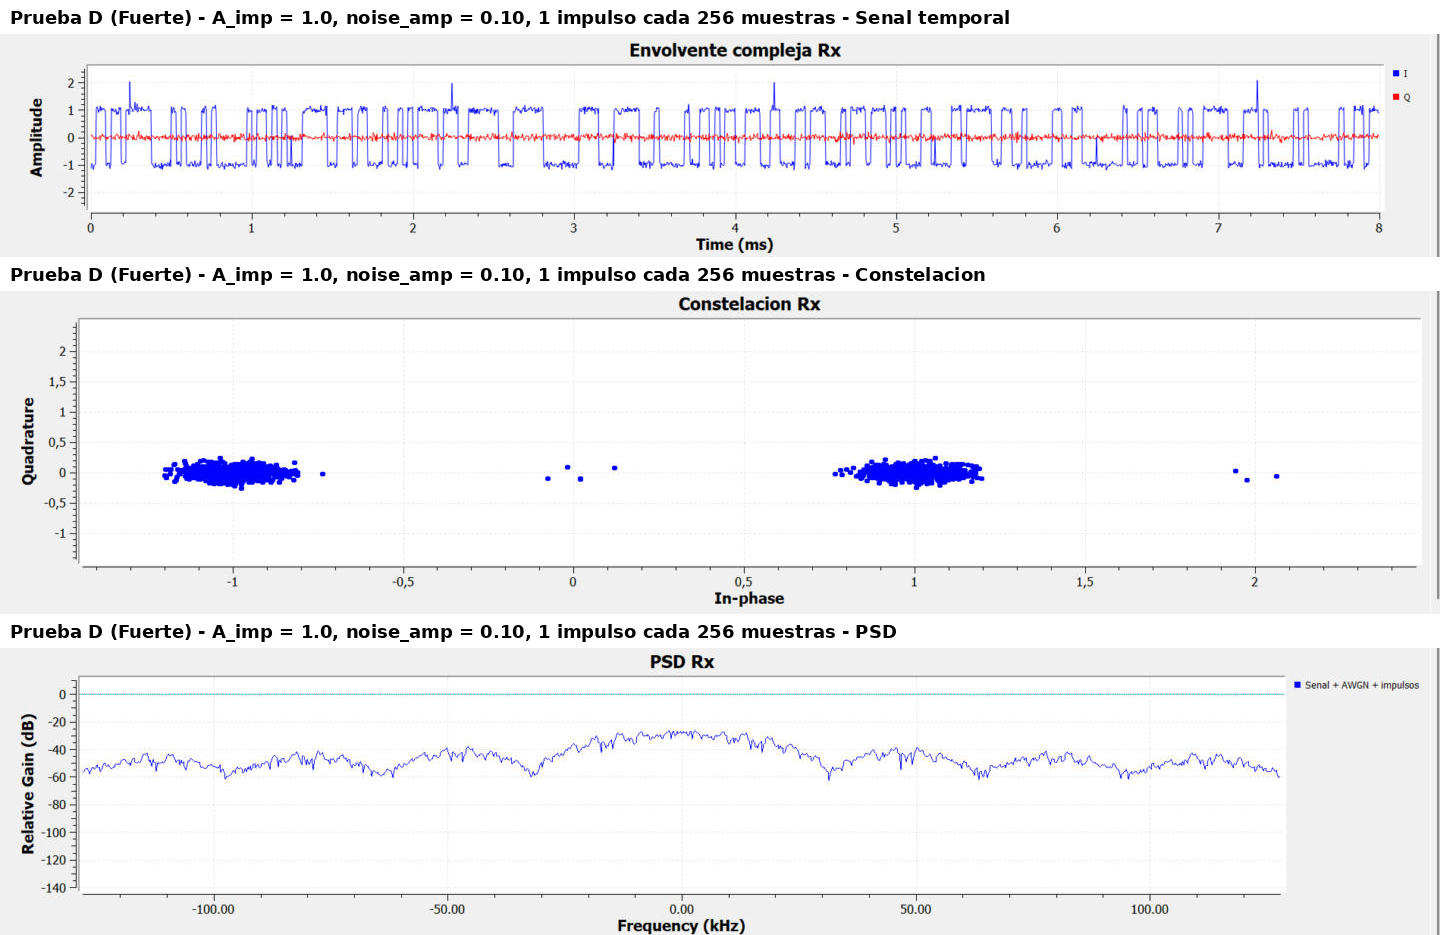
\includegraphics[width=0.82\textwidth]{Figuras/fase1_pruebaD.png}
    \caption{Fase~1, prueba D ($A_{imp}=1$, AWGN 0.10, pulso rectangular): envolvente compleja, constelación de las muestras y PSD a la salida del canal.}
    \label{fig:fase1}
\end{figure*}

\begin{table}[H]
    \centering
    \caption{Pruebas de la Fase 1 (pulso rectangular, sin receptor)}
    \label{tab:fase1}
    \footnotesize
    \setlength{\tabcolsep}{3pt}
    \begin{tabular}{@{}lcp{2.0cm}p{2.3cm}@{}}
        \toprule
        \textbf{Prueba} & $\mathbf{A_{imp}}$ & \textbf{Tiempo} & \textbf{Constelación} \\
        \midrule
        A (referencia) & 0.0 & niveles $\pm1$, sin picos & dos nubes en $\pm1$ \\
        B (suave) & 0.3 & picos de $\approx1.3$ cada 1 ms & puntos sueltos en $-0.7$ y $1.3$ \\
        C (media) & 0.6 & picos de $\approx1.6$ & puntos sueltos en $-0.4$ y $1.6$ \\
        D (fuerte) & 1.0 & picos de $\approx2$ & puntos sueltos en 0 y 2 \\
        \bottomrule
    \end{tabular}
\end{table}

La Fig.~\ref{fig:fase1} resume la prueba más severa. En el tiempo aparecen 8 picos en 8~ms, uno por milisegundo y solo en la componente I, porque el impulso es real. En la constelación, el AWGN abre cada símbolo en una nube, mientras que los impulsos producen unos pocos puntos aislados desplazados exactamente $+A_{imp}$ (una muestra de cada 256). La PSD conserva la forma $\mathrm{sinc}^2$ del pulso rectangular, con nulos en múltiplos de 32~kHz y unos 64~kHz entre primeros nulos, y casi no cambia entre pruebas: la potencia media del tren ($A_{imp}^2/256\le0.004$) es menor que la del AWGN (0.01). El hallazgo clave de esta fase es que, sin filtro acoplado, con $A_{imp}=1$ los puntos que venían del símbolo $-1$ caen en 0, justo en el umbral de decisión. Esto motivó dos decisiones de la Fase~2: conformar con RRC para reducir el ancho de banda y usar un filtro acoplado que reparta la energía del impulso antes de decidir.

\subsection{Fase 2: diseño y validación del sistema Tx--canal--Rx}
La Fig.~\ref{fig:flujograma} muestra el flujograma del enlace completo de la Fase~2. Las figuras de las secciones de espectro y receptor son capturas de ese flujograma en ejecución, con AWGN de amplitud 0.10 y la BER medida sobre una ventana de $10^5$ bits. Para los márgenes de decisión y como verificación de las curvas BER se usó además una simulación numérica que reproduce el flujograma bloque a bloque: los mismos 89 coeficientes RRC en Tx y Rx, el mismo retardo de 11 bits, la misma regla de decisión y la misma ley de inyección de ruido de la ecuación~\eqref{eq:pn}. Ambas coinciden: el flujograma midió BER $=0$ en las pruebas A a E y 0.2498 con 4 muestras de desfase, y la simulación dio 0 y 0.25.

Antes de las pruebas con perturbación, el receptor se validó en condición ideal, sin ruido ni impulsos (prueba 0, Anexo~\ref{app:capturas}). En ese caso la PSD del canal coincide con la del transmisor, la constelación recuperada se reduce a dos puntos exactos en $\pm1$ y la BER es cero: el filtro acoplado, el muestreo con desfase 0 y la referencia retrasada 11 bits funcionan sin errores antes de agregar el canal del proyecto.

\begin{figure*}[t]
    \centering
    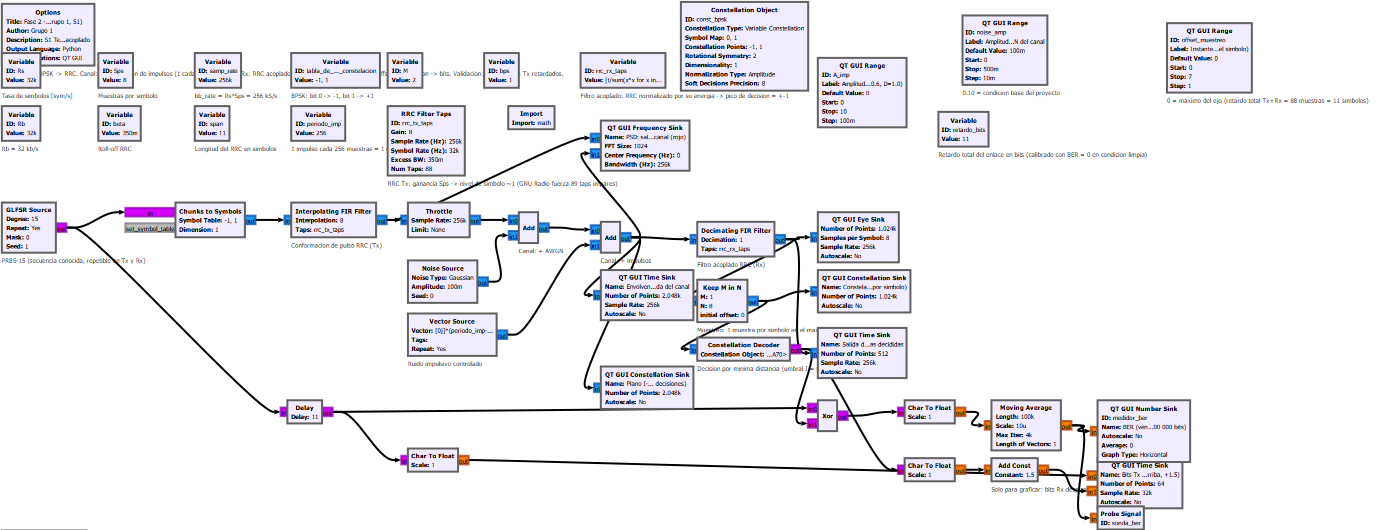
\includegraphics[width=0.95\textwidth]{Figuras/flujograma_fase2.png}
    \caption{Flujograma del enlace de la Fase~2: transmisor PRBS--BPSK--RRC, canal con AWGN y tren de impulsos, receptor con filtro acoplado, muestreo y decisión, y comparación de bits con la referencia retrasada 11 bits.}
    \label{fig:flujograma}
\end{figure*}

\subsubsection{Espectro y señal en el canal}
En la Fig.~\ref{fig:psd}, la señal a la salida del RRC del transmisor ocupa $\pm21.6$~kHz, como predice la ecuación~\eqref{eq:bw}, y fuera de esa banda sus lóbulos laterales caen más de 30~dB. Al agregar el canal, el AWGN fija un piso plano unos 30~dB por debajo de la banda de la señal. Con $A_{imp}=1$ el espectro casi no cambia respecto a la referencia: la potencia media del tren de impulsos es $1/256\approx0.004$, menos de la mitad de la del AWGN, y el piso sube apenas 1.5~dB (las capturas completas de todas las pruebas están en el Anexo~\ref{app:capturas}). Con $A_{imp}=5$ la potencia del tren es $25/256\approx0.098$, el piso sube unos 10~dB y aparece un peine de líneas separadas 1~kHz, que es la frecuencia de repetición de los impulsos (un impulso cada 256 muestras a 256~kS/s). La PSD, por ser un promedio, informa poco sobre el riesgo real: un evento de amplitud 5 en una sola muestra apenas se nota en ella.

\begin{figure*}[t]
    \centering
    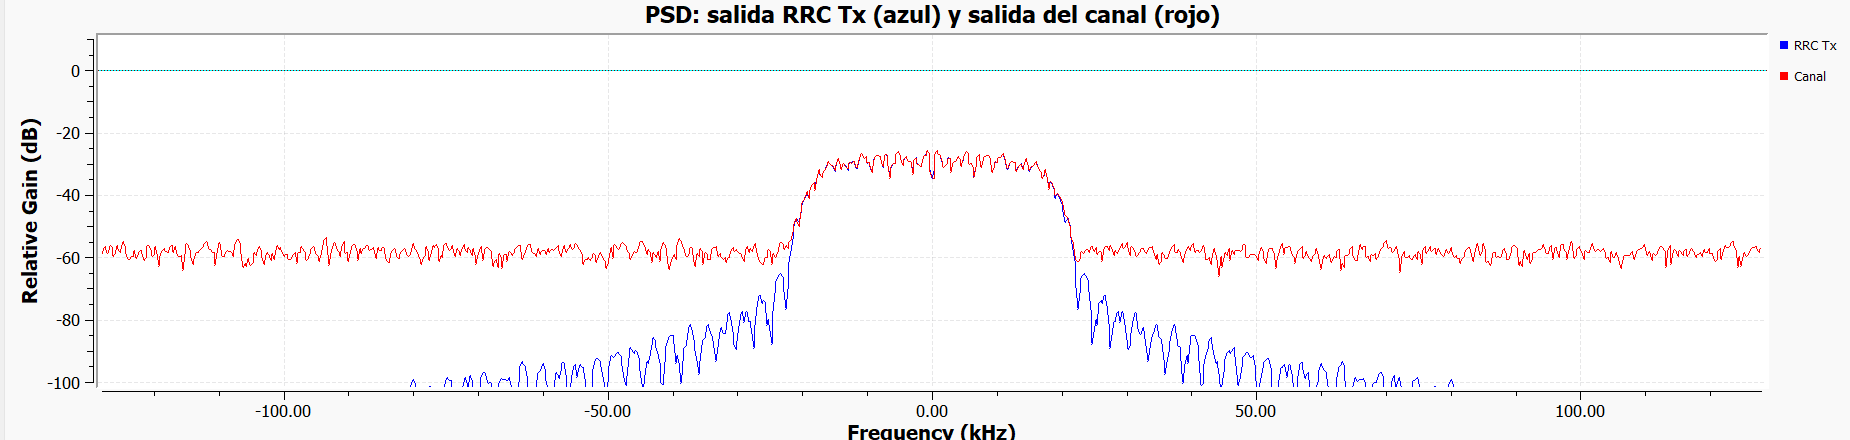
\includegraphics[width=0.49\textwidth]{Figuras/psd_A0.png}\hfill
    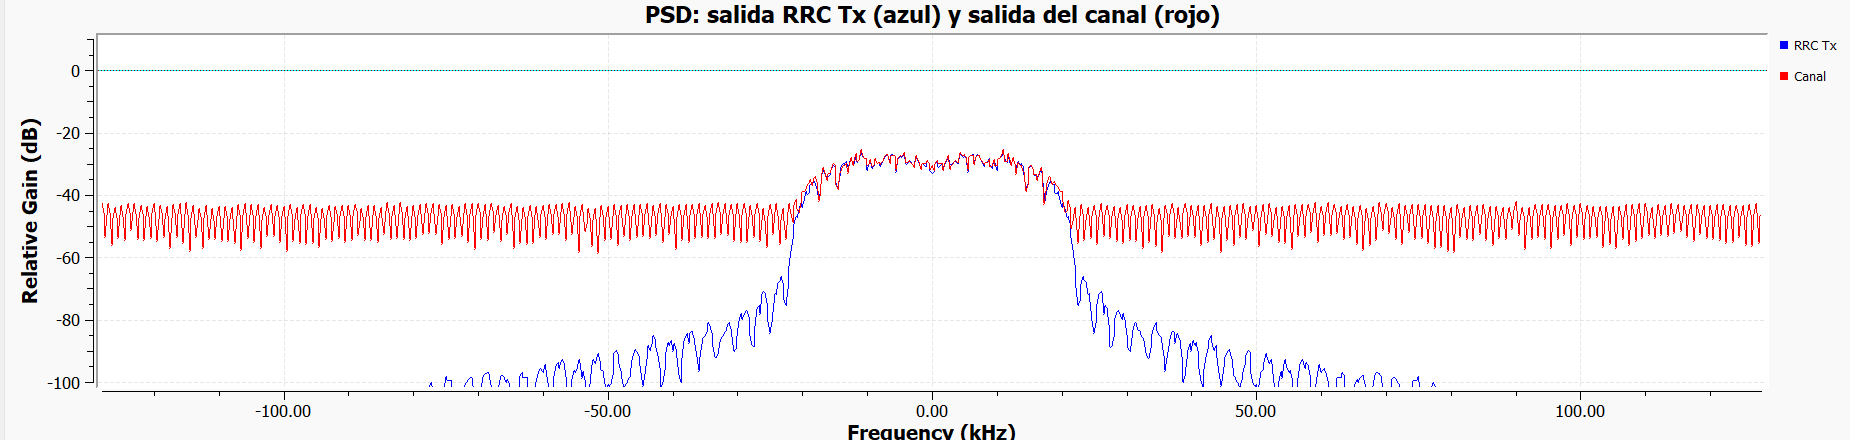
\includegraphics[width=0.49\textwidth]{Figuras/psd_A5.png}
    \caption{PSD a la salida del RRC del transmisor (azul) y a la salida del canal (rojo), con AWGN 0.10: prueba de referencia $A_{imp}=0$ (izquierda) y prueba de robustez $A_{imp}=5$ (derecha).}
    \label{fig:psd}
\end{figure*}

En el dominio del tiempo (Fig.~\ref{fig:tiempo}), en cambio, el impulso sí es visible: aparece solo en la componente I, porque es real, cada 1~ms. Su efecto depende del símbolo que coincide con él: sobre un nivel positivo produce un pico que supera 2, y sobre uno negativo reduce el nivel hacia cero.

\begin{figure}[H]
    \centering
    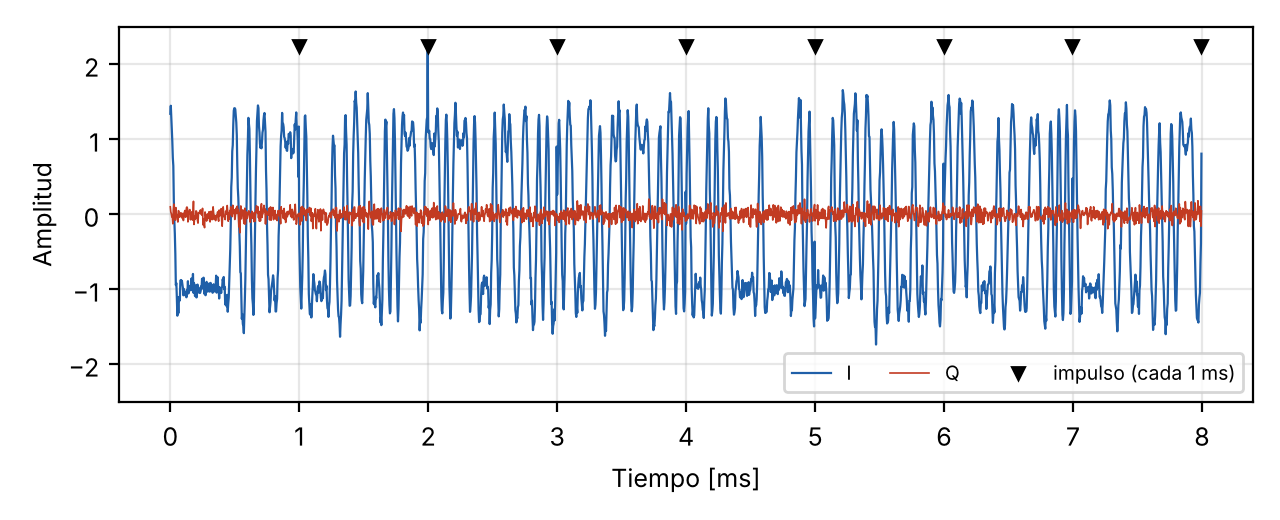
\includegraphics[width=\linewidth]{Figuras/tiempo_canal.png}
    \caption{Envolvente compleja a la salida del canal con $A_{imp}=1$ (8~ms; I en azul, Q en rojo). Los picos aislados de la componente I, uno por milisegundo, son los impulsos.}
    \label{fig:tiempo}
\end{figure}

\subsubsection{Receptor: ojo, constelación y bits}
La Fig.~\ref{fig:ojos} muestra el ojo a la salida del filtro acoplado. Con $A_{imp}=0$ las trayectorias convergen en $\pm1$ en los instantes de muestreo: la cascada RRC--RRC se comporta como un coseno alzado y no deja interferencia intersimbólica. Con $A_{imp}=0.6$ y $1.0$ el ojo es prácticamente el mismo. Solo con $A_{imp}=5$ aparecen trayectorias aisladas que se salen del haz, y aun así el ojo sigue abierto en el centro.

\begin{figure}[H]
    \centering
    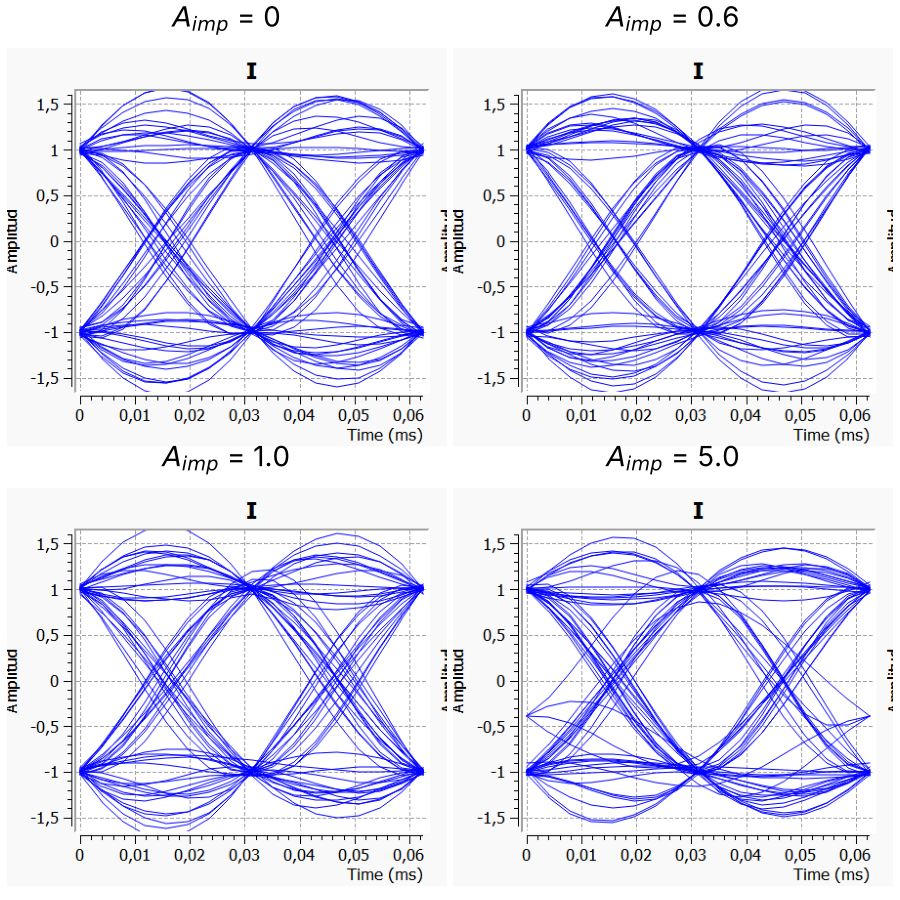
\includegraphics[width=\linewidth]{Figuras/ojos.png}
    \caption{Diagramas de ojo a la salida del filtro acoplado (componente I, dos símbolos).}
    \label{fig:ojos}
\end{figure}

La explicación está en el filtro acoplado. Un impulso de una muestra no se suma de forma directa a la variable de decisión: sale del filtro convertido en la forma del pulso, escalado por $1/\sum h^2$. Como el período de 256 muestras es múltiplo de SPS~$=8$, el impulso cae siempre en la misma fase dentro del símbolo, y en los instantes de muestreo su contribución máxima es $0.100\,A_{imp}$ (algo menor que la cota de 0.137 de la ecuación~\eqref{eq:atenuacion}, que corresponde al pico del pulso). Con $A_{imp}=1$ la muestra más afectada se corre $0.10$, frente a una distancia de 1 al umbral. Por eso la constelación recuperada (Fig.~\ref{fig:const}) mantiene dos nubes compactas en $\pm1$ hasta $A_{imp}=1$. Con $A_{imp}=5$ aparecen dos grupos de puntos aislados, cerca de $-0.5$ y $+1.5$: son los símbolos que coinciden con el impulso, desplazados $+0.5$ hacia la derecha porque el impulso es positivo. Con 4 muestras de desfase, en cambio, los puntos se reparten a lo largo de todo el eje I y la BER sube a 0.25.

\begin{figure}[H]
    \centering
    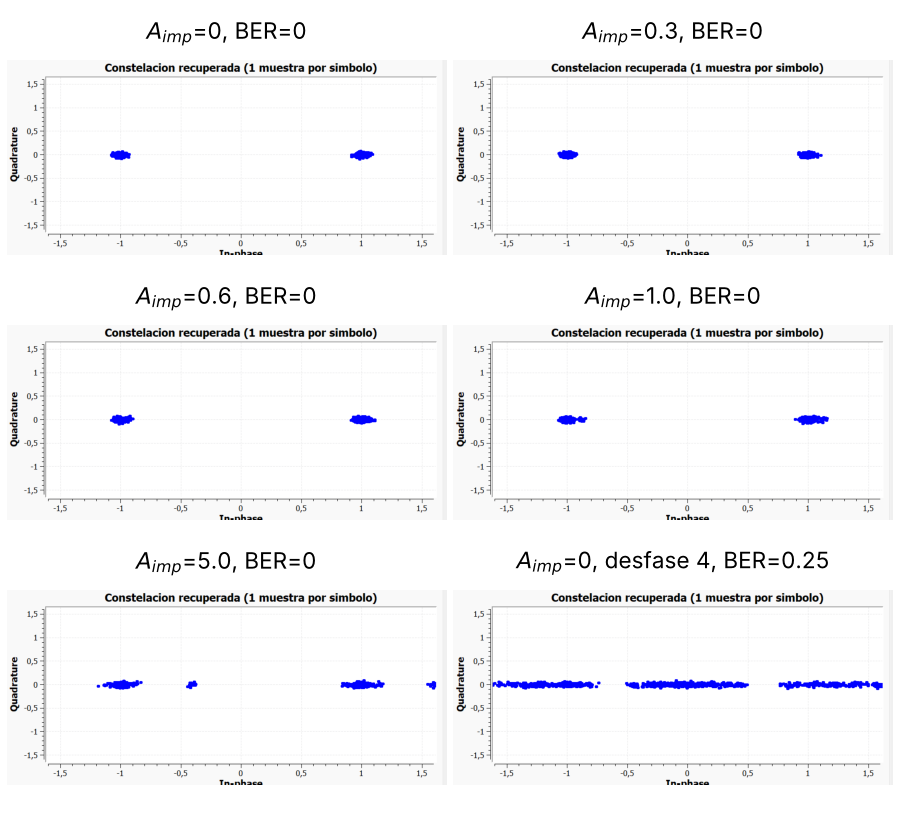
\includegraphics[width=\linewidth]{Figuras/constelaciones.png}
    \caption{Constelación recuperada (una muestra por símbolo): condición ideal, cada amplitud de impulso con AWGN 0.10 y, en el último panel, el efecto de muestrear con 4 muestras de desfase.}
    \label{fig:const}
\end{figure}

La Tabla~\ref{tab:fase2} resume la validación. En todas las pruebas los bits recuperados coinciden con los transmitidos una vez se compensan los 11 bits de retardo (Fig.~\ref{fig:bits}). El margen mínimo, es decir el menor $|I|$ observado en las muestras de decisión, cae de 0.88 a 0.40 cuando $A_{imp}$ pasa de 0 a 5. Sin AWGN, el primer error aparecería cuando $0.100\,A_{imp}>1$, es decir para $A_{imp}\approx10$.

\begin{table}[H]
    \centering
    \caption{Validación del receptor (AWGN 0.10 salvo en la prueba 0): BER medida en el flujograma (ventana de $10^5$ bits) y margen mínimo de la simulación ($2\times10^5$ bits)}
    \label{tab:fase2}
    \footnotesize
    \begin{tabular}{@{}lccc@{}}
        \toprule
        \textbf{Prueba} & $\mathbf{A_{imp}}$ & \textbf{BER} & \textbf{Margen mínimo $|I|$} \\
        \midrule
        0 (ideal, sin ruido) & 0.0 & 0 & 0.99 \\
        A (referencia) & 0.0 & 0 & 0.88 \\
        B (suave) & 0.3 & 0 & 0.88 \\
        C (media) & 0.6 & 0 & 0.85 \\
        D (fuerte) & 1.0 & 0 & 0.81 \\
        E (robustez) & 5.0 & 0 & 0.40 \\
        F (desfase 4) & 0.0 & 0.2498 & -- \\
        \bottomrule
    \end{tabular}
\end{table}

\begin{figure}[H]
    \centering
    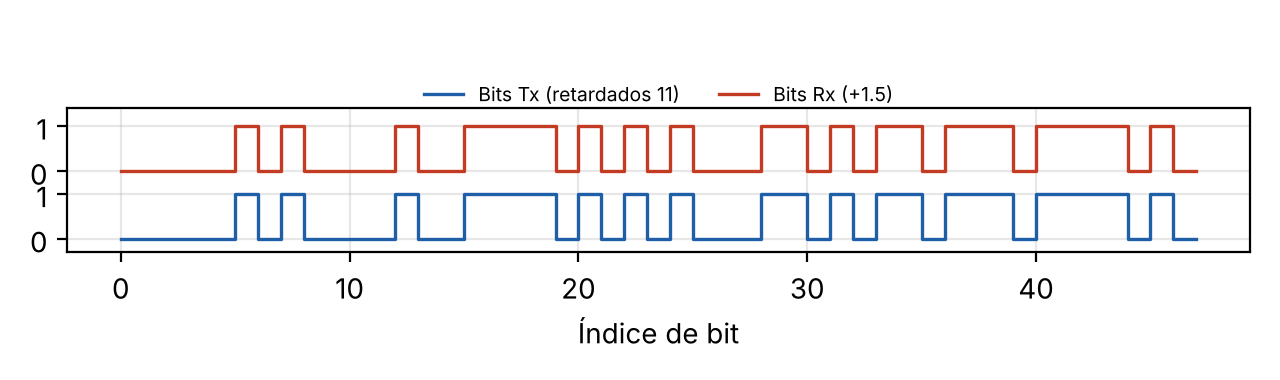
\includegraphics[width=\linewidth]{Figuras/bits_tx_rx.png}
    \caption{Bits transmitidos (abajo, retrasados 11 bits) y bits recuperados (arriba, desplazados $+1.5$) con $A_{imp}=1$.}
    \label{fig:bits}
\end{figure}

El instante de muestreo resultó tan determinante como el canal. Con el desfase correcto (0 muestras) el margen es 0.88; con 2 muestras de error baja a 0.18, y con 4 muestras ---el cruce del ojo--- la BER sube a 0.25 sin que el canal haya cambiado. Este resultado justifica calcular el retardo total del enlace (88 muestras, 11 símbolos) antes de fijar el muestreo y, en hardware, recuperar el reloj de forma adaptativa.

\subsection{Fase 3: configuración de la interfaz SDR}
En la tercera fase el enlace se llevó a flujogramas para HackRF One y USRP (Fig.~\ref{fig:fase3flujos}). El transmisor conserva la fuente PRBS-15, la codificación diferencial, el mapeo BPSK y el RRC de la Fase~2; después del RRC se agregan un factor de amplitud digital (para mantener el pico por debajo de 1 y no saturar el conversor), la adaptación de tasa a la del radio, el desplazamiento del oscilador y el bloque del radio. El receptor invierte el camino: corrige el desplazamiento del oscilador, vuelve a 256~kS/s y suma de forma digital el mismo tren de impulsos del proyecto, para reproducir el escenario sobre la señal real. Como los dos radios tienen osciladores independientes, agrega control automático de ganancia, lazo de frecuencia de borde de banda (corrige el offset entre osciladores), sincronización de reloj con banco polifásico de filtros RRC (que cumple además la función del filtro acoplado y elige el instante de muestreo de forma adaptativa) y lazo de Costas de orden 2, antes de la misma decisión y decodificación diferencial. Un filtro RRC adicional alimenta solo el diagrama de ojo de diagnóstico. Se eliminó el bloque de regulación de ritmo y el modelo de canal: con hardware, el radio fija el ritmo de muestras y el canal es el medio físico.

\begin{figure*}[!t]
    \centering
    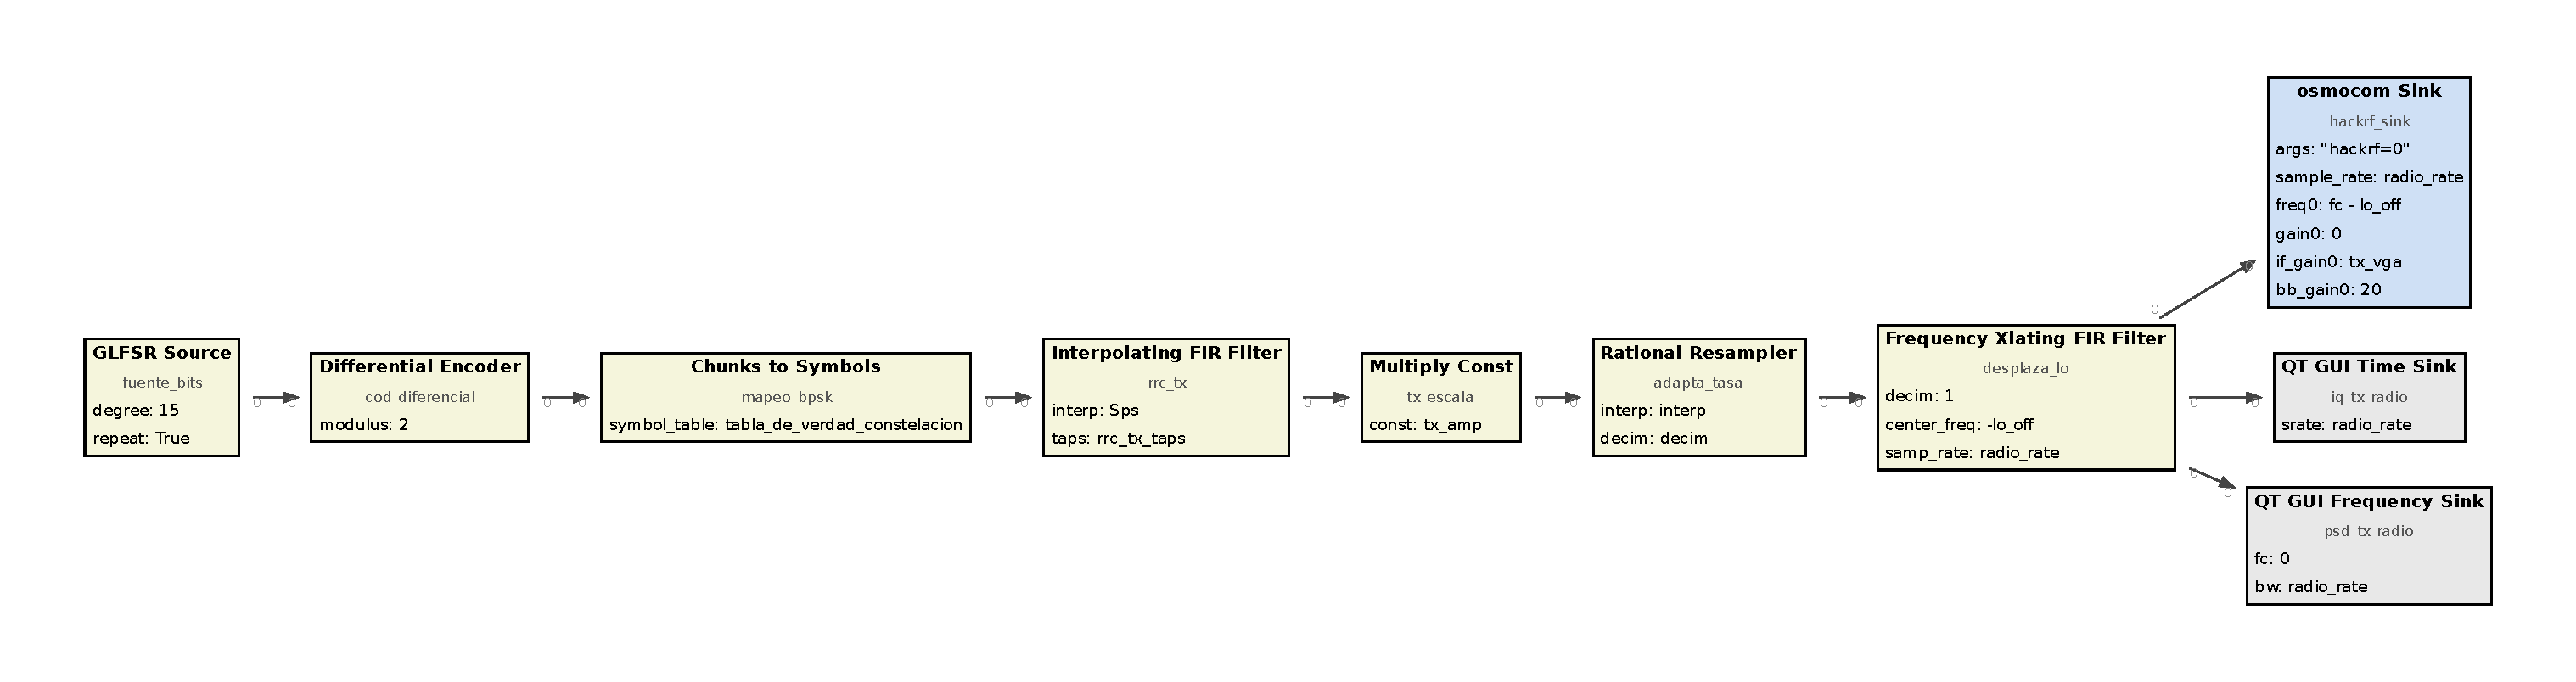
\includegraphics[width=0.92\textwidth]{Figuras/fase3_tx.pdf}\\[2mm]
    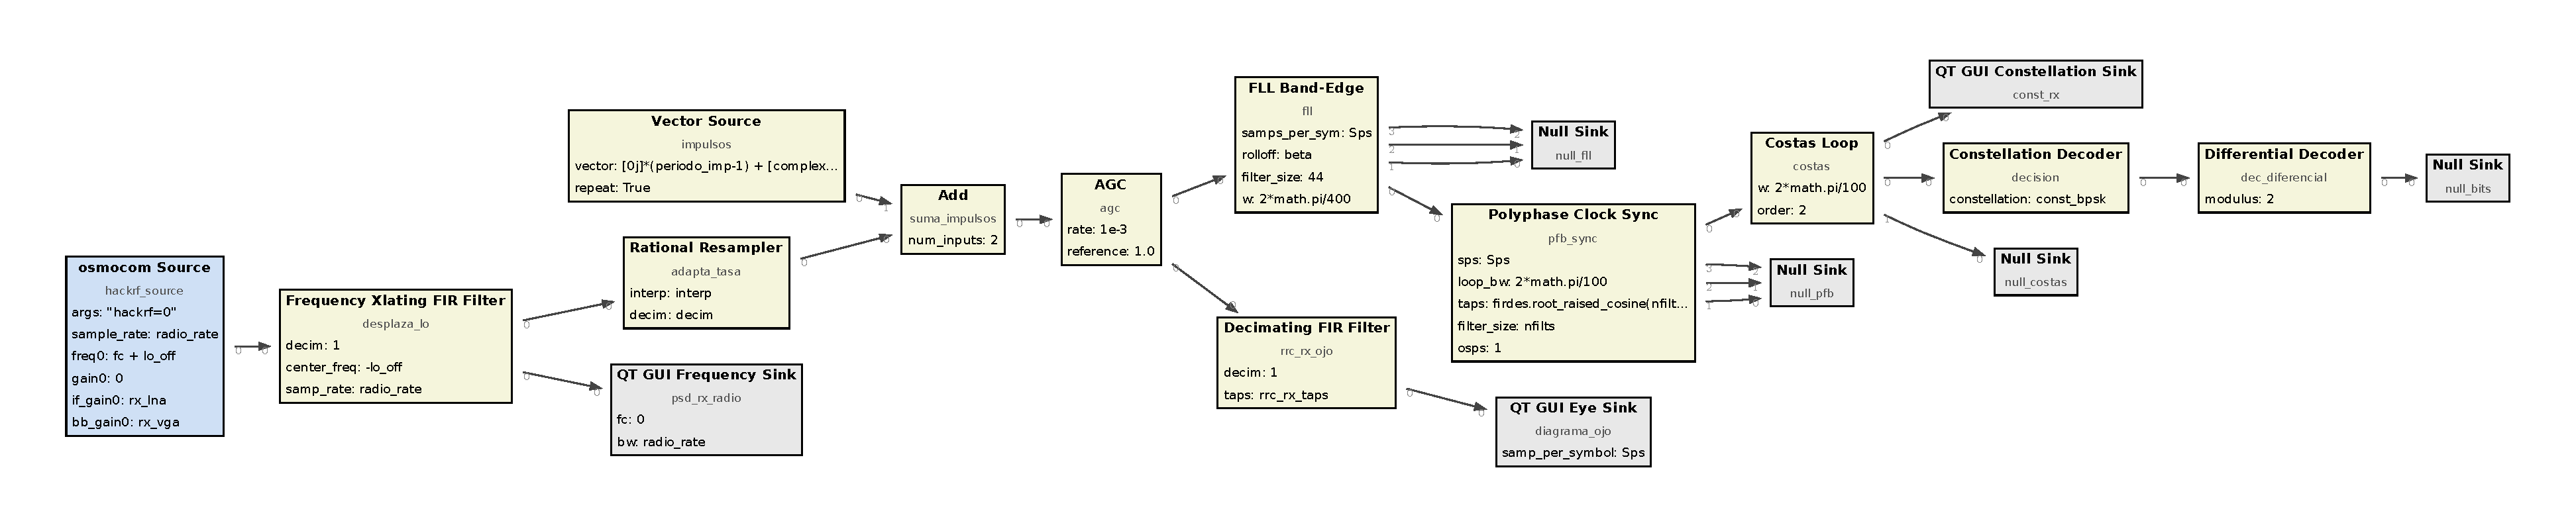
\includegraphics[width=\textwidth]{Figuras/fase3_rx.pdf}
    \caption{Flujogramas de la Fase~3 para HackRF One, con los parámetros principales de cada bloque tomados de los archivos \texttt{.grc}. Arriba, transmisor: PRBS, codificación diferencial, BPSK, RRC, amplitud, remuestreo a 2~MS/s, desplazamiento del oscilador y \textit{osmocom Sink}. Abajo, receptor: \textit{osmocom Source}, corrección del oscilador, regreso a 256~kS/s, suma de impulsos, AGC, FLL, sincronización de reloj polifásica, Costas, decisión y decodificación diferencial. Las versiones para USRP solo cambian el bloque del radio (UHD) y la tasa (1~MS/s).}
    \label{fig:fase3flujos}
\end{figure*}


La Fig.~\ref{fig:bloques} muestra la configuración de los bloques de radio y la Tabla~\ref{tab:sdr} (Anexo~\ref{app:sdr}) justifica cada parámetro. La separación entre diseño y hardware es la idea central de esta fase. Modulación, $R_s$, $R_b$, SPS, $\beta$, span, mapeo y decisión pertenecen al diseño de comunicaciones y no cambiaron. Frecuencia central (960~MHz), tasa del radio (2~MS/s en HackRF, 1~MS/s en USRP), remuestreo racional ($\times125/16$ y $\times125/32$), ganancias, ancho de banda RF, puerto, reloj y desplazamiento de 200~kHz del oscilador pertenecen a la interfaz. Así, cualquier diferencia entre la simulación y la medición en hardware se puede atribuir a la interfaz y al medio físico, y no a un cambio del diseño.

\begin{figure*}[t]
    \centering
    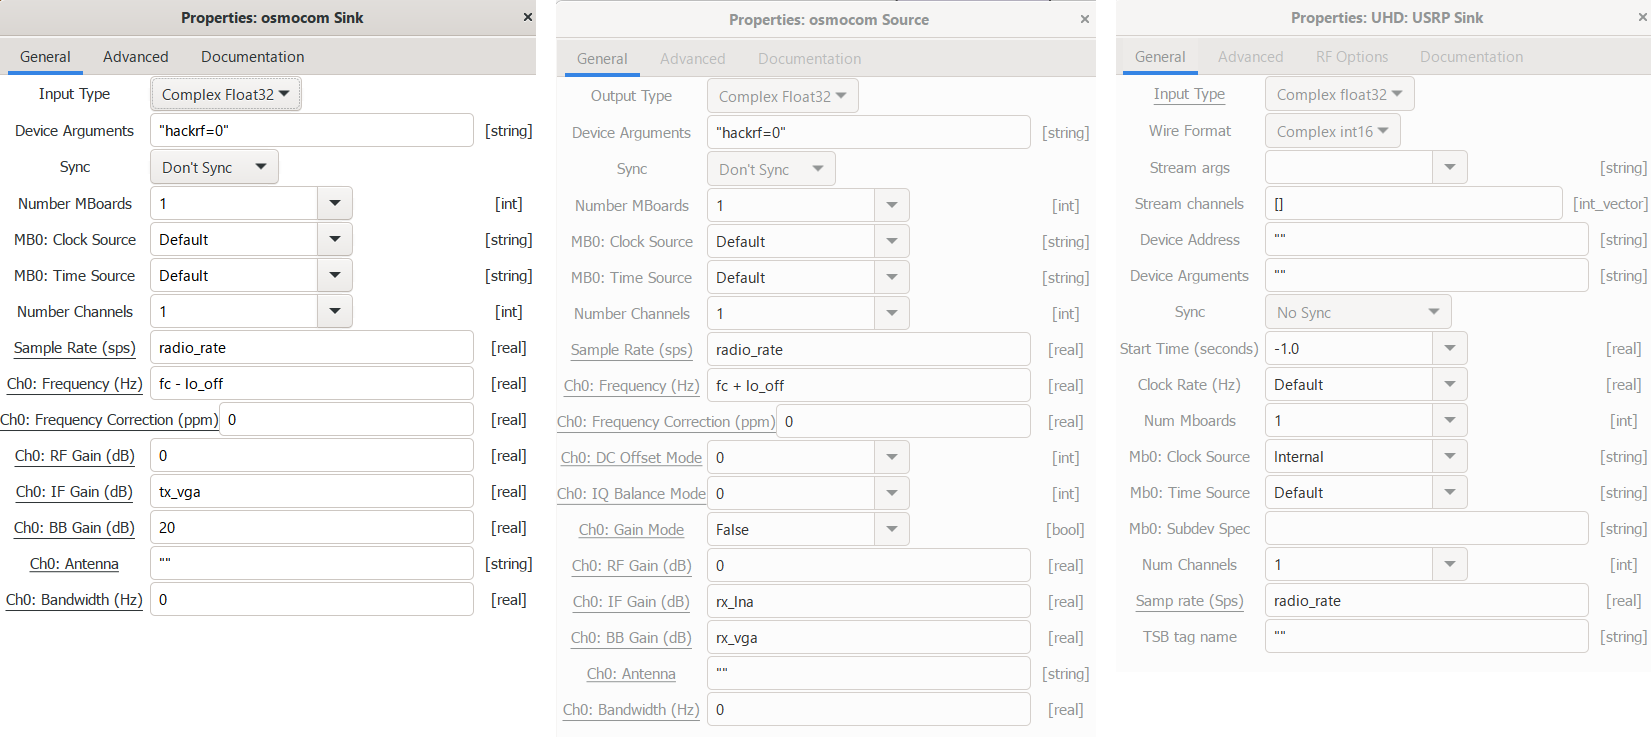
\includegraphics[width=\textwidth]{Figuras/bloques_radio.png}
    \caption{Configuración de los bloques de radio: Osmocom Sink (transmisor HackRF), Osmocom Source (receptor HackRF) y UHD: USRP Sink (transmisor USRP).}
    \label{fig:bloques}
\end{figure*}

En el Osmocom Sink la frecuencia es \texttt{fc - lo\_off}, la tasa \texttt{radio\_rate}, la ganancia de RF (amplificador) 0 y la ganancia IF \texttt{tx\_vga}; el campo BB no tiene efecto en transmisión con HackRF. En el Osmocom Source la frecuencia es \texttt{fc + lo\_off}, la ganancia IF corresponde al LNA (\texttt{rx\_lna}) y la BB al VGA (\texttt{rx\_vga}), con el control automático de ganancia del radio desactivado para que el nivel sea repetible. En ambos, el ancho de banda 0 deja que el driver elija el filtro analógico. En el USRP Sink la dirección vacía toma el primer equipo encontrado, el reloj es interno y la frecuencia, la ganancia y la antena (TX/RX) se fijan en la pestaña de opciones de RF.

\begin{figure*}[t]
    \centering
    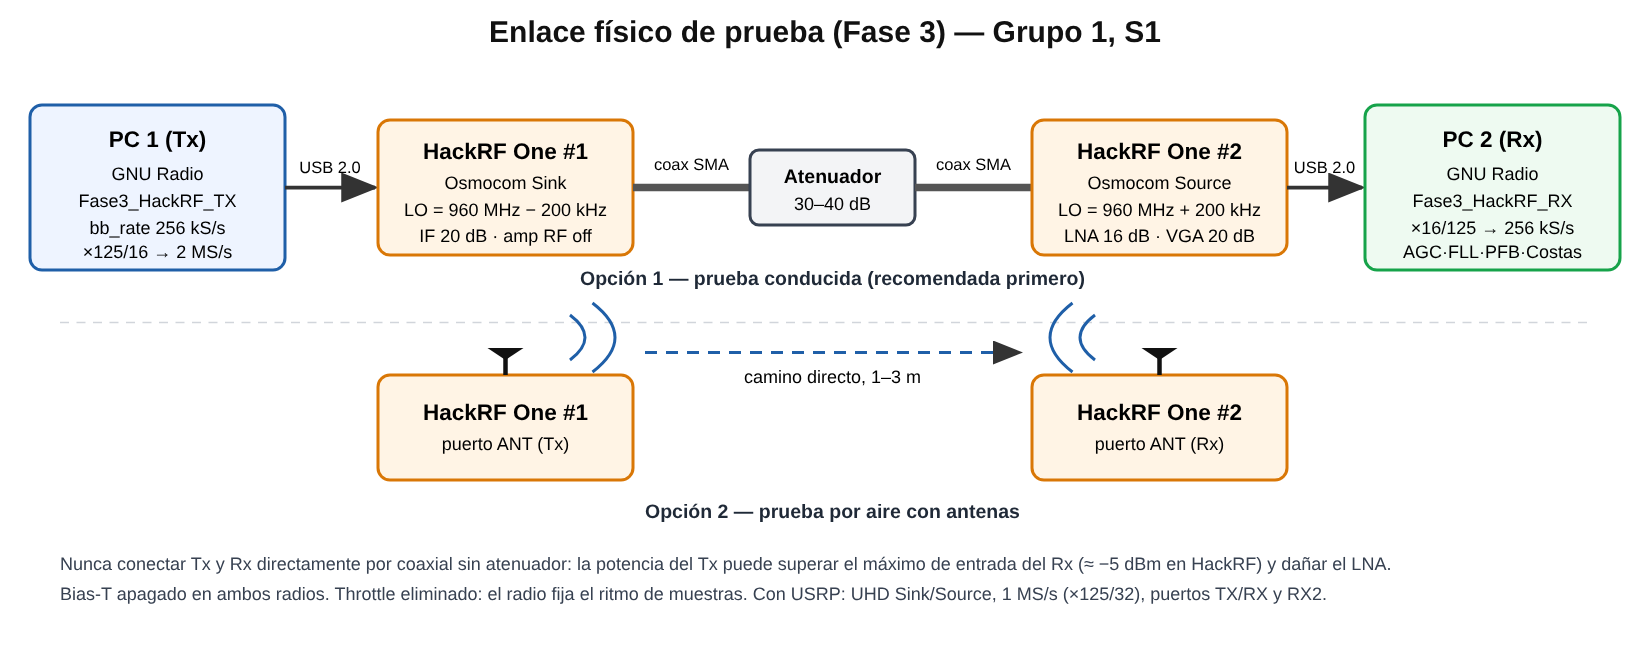
\includegraphics[width=0.9\textwidth]{Figuras/enlace_fisico.png}
    \caption{Montaje del enlace físico de prueba: por cable con atenuador (opción 1) o por aire con antenas (opción 2).}
    \label{fig:enlace}
\end{figure*}

La Fig.~\ref{fig:enlace} muestra el montaje previsto. La primera prueba se hace por cable con al menos 30~dB de atenuación, porque la potencia del transmisor puede superar el máximo de entrada del receptor (unos $-5$~dBm en HackRF). La tasa de bits no depende del radio: $256\,000\times125/16=2\times10^6$ muestras/s, y la señal de 43~kHz queda muy por debajo del ancho de banda del radio. Para medir la BER en hardware, \texttt{delay\_bits} se calibra primero con el bloque del Anexo~\ref{app:retardo}, porque el retardo deja de ser 11 bits: depende de los remuestreadores, de la sincronización y del instante en que arrancan el transmisor y el receptor. Los errores encontrados durante la configuración y su solución están en la Tabla~\ref{tab:errores}.

\subsection{Fase 4: validación con curvas BER}
Las curvas de la Fig.~\ref{fig:ber} se midieron en los flujogramas de la Fase~4 con el instrumento del curso, con los parámetros de la Tabla~\ref{tab:instr}: \texttt{e\_EbN0\_Sweep} se ubicó a la salida del canal, justo antes del filtro acoplado, y \texttt{e\_BER\_Curve} recibe los bits de la fuente PRBS (entrada 0) y los bits a la salida del decodificador diferencial (entrada 1) (Anexo~\ref{app:fase4}).

\begin{table}[H]
    \centering
    \caption{Parámetros del instrumento BER}
    \label{tab:instr}
    \footnotesize
    \begin{tabular}{@{}ll@{}}
        \toprule
        \textbf{Parámetro} & \textbf{Valor} \\
        \midrule
        $R_b$ & 32\,000 b/s \\
        \texttt{bb\_rate} (entrada del receptor) & 256\,000 muestras/s \\
        \texttt{EbN0\_min} / \texttt{EbN0\_max} / \texttt{EbN0\_step} & 0 / 14 / 1 dB \\
        \texttt{bits\_por\_punto} / \texttt{bits\_guardia} & 100\,000 / 1000 \\
        \texttt{delay\_bits} & 11 \\
        \texttt{update\_every} & 1000 \\
        \bottomrule
    \end{tabular}
\end{table}

Para alinear Tx y Rx se partió del retardo calculado en la Fase~2 (88 muestras = 11 símbolos) y se verificó con el bloque \texttt{e\_Busca\_Retardo}, que correlaciona ambas secuencias en una condición limpia. Cada flujograma corrió 4 minutos, unas 15 vueltas del barrido, lo que da entre $1.4$ y $1.6\times10^6$ bits por punto. Antes de medir, el bloque \texttt{e\_Busca\_Retardo} confirmó el retardo de 11 bits con correlación $+1.000$ y BER nula en los puntos de alta $E_b/N_0$.

Sin impulsos, la curva coincide con la de BPSK con codificación diferencial: $E_b/N_0=7.30$~dB para BER $=10^{-3}$, frente a 7.33~dB teóricos y 6.79~dB de BPSK coherente sin codificación diferencial. Esa diferencia de unos 0.5~dB es el costo de resolver la ambigüedad de fase, porque un error de símbolo produce dos errores de bit consecutivos. Con $A_{imp}=1$ la curva prácticamente no se distingue de la referencia (7.38~dB), lo que confirma lo observado en el ojo. Los pocos errores registrados a 14~dB en esas dos curvas (unos 10 en $1.4\times10^6$ bits) no son del enlace: aparecen en el salto de 14 a 0~dB al reiniciar el barrido, cuando algunos bits del final del punto de 14~dB ya reciben el ruido del punto de 0~dB. A 12 y 13~dB no hubo errores.

\begin{figure}[H]
    \centering
    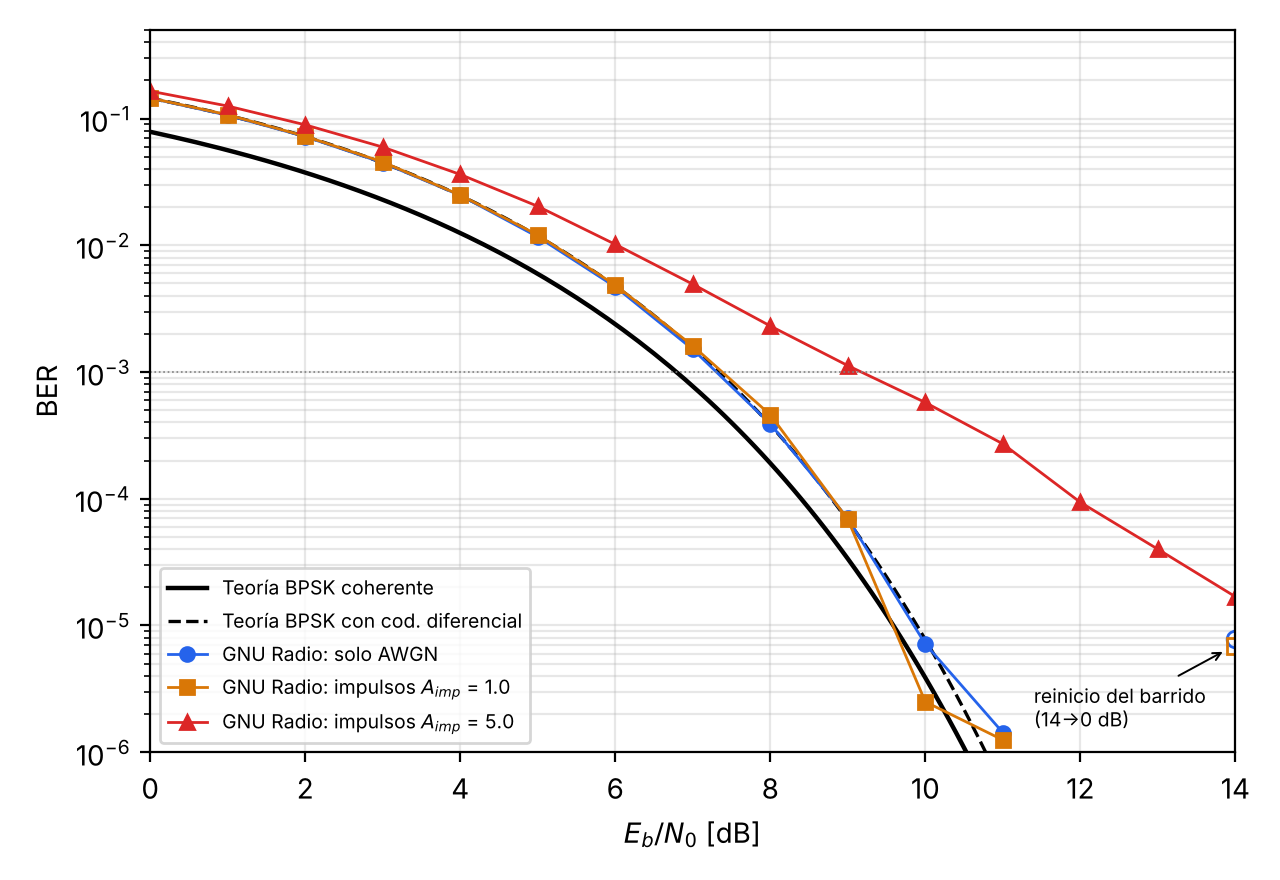
\includegraphics[width=\linewidth]{Figuras/curva_ber.png}
    \caption{BER frente a $E_b/N_0$ medida en los flujogramas de la Fase~4 ($A_{imp}=0$, 1 y 5) junto con la teoría de BPSK coherente y con codificación diferencial. Los puntos vacíos a 14~dB son errores causados por el reinicio del barrido.}
    \label{fig:ber}
\end{figure}

Con $A_{imp}=5$ la curva se separa: requiere 9.17~dB para BER $=10^{-3}$ (1.8~dB más que la referencia) y, en lugar de caer en forma de cascada, decrece lentamente: $2.7\times10^{-4}$ a 11~dB y $1.7\times10^{-5}$ a 14~dB. El comportamiento se explica con un modelo simple. De cada 32 símbolos, el más cercano al impulso pierde la mitad de su distancia al umbral ($1-0.100\times5=0.5$), es decir, unos 6~dB de relación señal a ruido, y a alta $E_b/N_0$ son esos símbolos los que producen casi todos los errores. Promediando la probabilidad de error de cada símbolo según su desplazamiento se obtienen $1.1\times10^{-3}$ a 9~dB y $2.7\times10^{-4}$ a 11~dB; el flujograma midió $1.12\times10^{-3}$ y $2.71\times10^{-4}$, y la simulación numérica del mismo enlace dio valores iguales. Parte de la penalización, unos 0.4~dB, es aparente: el instrumento mide la potencia recibida incluyendo los impulsos y asigna ruido con base en ella.

\begin{table}[H]
    \centering
    \caption{$E_b/N_0$ requerido para BER $=10^{-3}$}
    \label{tab:ber}
    \footnotesize
    \begin{tabular}{@{}lcc@{}}
        \toprule
        \textbf{Condición} & $\mathbf{E_b/N_0}$ \textbf{[dB]} & \textbf{Penalización [dB]} \\
        \midrule
        Teoría BPSK coherente & 6.79 & -- \\
        Teoría con cod. diferencial & 7.33 & referencia \\
        Medido, sin impulsos & 7.30 & $-0.03$ \\
        Medido, $A_{imp}=1$ & 7.38 & $+0.05$ \\
        Medido, $A_{imp}=5$ & 9.17 & $+1.84$ \\
        \bottomrule
    \end{tabular}
\end{table}


La curva medida sin impulsos es la referencia contra la que se compara la curva experimental con el radio, con el criterio del curso de una penalización máxima de 2~dB en BER $=10^{-3}$.
